\documentclass[12pt,a4paper]{article}

% ================= PACKAGES =================
\usepackage[margin=1in]{geometry}
\usepackage[T1]{fontenc}
\usepackage{graphicx}
\usepackage{titlesec}
\usepackage{tabularx}
\usepackage{longtable}
\usepackage{array}
\usepackage{hyperref}
\usepackage{xurl}
\usepackage{needspace}
\usepackage{listings}
\usepackage{xcolor}
\usepackage{enumitem}
\usepackage{setspace}
\usepackage[most]{tcolorbox}
\usepackage{mathptmx}   % Times New Roman-equivalent font, applies to entire document

% ================= FONT SIZE LADDER =================
% Absolute sizes so nothing depends on class-relative scaling.
\newcommand{\sizeEighteen}{\fontsize{18pt}{22pt}\selectfont}  % \section
\newcommand{\sizeSixteen}{\fontsize{16pt}{20pt}\selectfont}   % \subsection
\newcommand{\sizeFourteen}{\fontsize{14pt}{17pt}\selectfont}  % \subsubsection
\newcommand{\sizeTwelve}{\fontsize{12pt}{14.5pt}\selectfont}  % body / minimum

% ================= HEADER COLORS =================
\definecolor{RamaiahBlue}{RGB}{27,31,92}
\definecolor{RamaiahMaroon}{RGB}{139,30,63}

% ================= CODE LISTING STYLE =================
% basicstyle and numberstyle both forced to 12pt -- nothing prints smaller.
% xleftmargin keeps the 12pt line numbers inside the A4 text block.
\lstdefinestyle{codestyle}{
    backgroundcolor=\color{black!5},
    commentstyle=\color{green!50!black},
    keywordstyle=\color{blue},
    stringstyle=\color{orange},
    basicstyle=\ttfamily\fontsize{12pt}{14.4pt}\selectfont,
    numberstyle=\ttfamily\fontsize{12pt}{14.4pt}\selectfont,
    breaklines=true,
    breakatwhitespace=false,
    frame=single,
    numbers=left,
    numbersep=8pt,
    xleftmargin=3.2em,
    aboveskip=10pt,
    belowskip=10pt,
    showstringspaces=false
}
\lstset{style=codestyle,columns=fullflexible,keepspaces=true}

% ================= HEADING FORMATS =================
\titleformat{\section}{\sizeEighteen\bfseries}{\thesection}{1em}{}
\titleformat{\subsection}{\sizeSixteen\bfseries}{\thesubsection}{1em}{}
\titleformat{\subsubsection}{\sizeFourteen\bfseries}{\thesubsubsection}{1em}{}

\titlespacing*{\section}{0pt}{18pt}{10pt}
\titlespacing*{\subsection}{0pt}{16pt}{8pt}
\titlespacing*{\subsubsection}{0pt}{14pt}{7pt}

% ================= REPEATABLE HEADER BANNER =================
\newcommand{\reportheader}{%
\noindent
\begin{minipage}[c]{0.38\textwidth}
  
\includegraphics[height=1.2cm]{ramaiah_logo.jpg}
\end{minipage}%
\begin{minipage}[c]{0.62\textwidth}
  \raggedleft
  {\color{RamaiahBlue}\sizeFourteen\bfseries Department of CSE (Artificial Intelligence \& Machine Learning) and CSE (Cyber Security)}
\end{minipage}\\[0.2cm]
\noindent\textcolor{RamaiahMaroon}{\rule{\linewidth}{1.2pt}}
\vspace{0.4cm}
}

\graphicspath{{../../evidences/}{evidences/}{./}}
\hypersetup{pdfauthor={Syed Shaibaan Hussain},pdftitle={DevOps Self Learning Activity Report - Unit Converter API},breaklinks=true}
\begin{document}
\pagestyle{empty}
\sizeTwelve

\reportheader

\vspace{1.0cm}
\begin{center}
{\sizeEighteen \bfseries SELF LEARNING ACTIVITY REPORT \par}

\vspace{1.2cm}

{\sizeTwelve Submitted in partial fulfilment of the Requirements for \\[0.2cm]
the Academics of 5\textsuperscript{th} Semester, B.E in CSE (Cyber Security) \par}

\vspace{1.2cm}

{\sizeEighteen \bfseries DEVOPS \par}

\vspace{0.5cm}

{\sizeSixteen \bfseries 25CYAEC59 \par}

\vspace{1.2cm}

{\sizeTwelve In \par}

\vspace{0.45cm}

{\sizeFourteen \bfseries Dept. of CSE (CYBER SECURITY) \par}

\vspace{1.2cm}

{\sizeTwelve By \par}

\vspace{0.4cm}

{\sizeFourteen \bfseries Syed Shaibaan Hussain \\[0.15cm] USN: 1MS24CY056 \par}

\vspace{1.5cm}

{\sizeTwelve Under the guidance of \par}
\vspace{0.3cm}

{\sizeFourteen \bfseries Mr. Prashanth Reddy C \par}
\vspace{0.15cm}

{\sizeTwelve Senior Lecturer \par}
{\sizeTwelve Department of CSE (AI \& ML) and CSE (Cyber Security) \par}

\vspace{1.5cm}

{\sizeSixteen \bfseries M. S. Ramaiah Institute of Technology \par}
\vspace{0.3cm}
{\sizeTwelve (Autonomous Institute Affiliated to VTU) \\ MSR Nagar, MSRIT Post \par}
\vspace{0.1cm}
{\sizeTwelve Bangalore-560054, Karnataka, India \par}
\end{center}

\newpage

% ======================================================

\reportheader

\vspace{1.0cm}
\begin{center}
{\sizeEighteen \bfseries Certificate \par}
\end{center}

\vspace{0.8cm}

\noindent
{\sizeTwelve
This is to certify that the work carried out is a bonafide record of the project based learning activity work on the DevOps course done by Syed Shaibaan Hussain (1MS24CY056) under my supervision and guidance, in partial fulfilment of the requirements for the award of the Bachelor of Engineering in Computer Science \& Engineering (Cyber Security) from Ramaiah Institute of Technology, Bangalore for the academic year 2026-2027.
\par}

\vspace{3.5cm}

\noindent
{\sizeTwelve Candidate Sign \hfill Faculty Sign \par}

\newpage
\pagestyle{plain}

% ======================================================

\section*{LIST OF PROJECT BASED LEARNING COMPONENTS}

\noindent
{\sizeTwelve
\textbf{COURSE NAME:} DevOps \hfill \textbf{COURSE CODE:} 24CYAEC59 \\
\textbf{CREDITS:} 1:0:0 \hfill \textbf{CONTACT HOURS:} 15L \\
\textbf{MAX. MARKS:} 20
\par}

\vspace{0.6cm}

{\sizeTwelve
\setlength{\tabcolsep}{4pt}
\renewcommand{\arraystretch}{1.25}
\begin{longtable}{|>{\centering\arraybackslash}m{1.2cm}|>{\raggedright\arraybackslash}p{10.6cm}|>{\centering\arraybackslash}m{1.8cm}|}
\hline
\multicolumn{1}{|c|}{\textbf{Sl. No}} &
\multicolumn{1}{c|}{\textbf{Description}} &
\multicolumn{1}{c|}{\textbf{Marks}} \\
\hline
\endhead

1 &
\textbf{CI/CD Pipeline using Git, Maven/Gradle and Jenkins.}
Set up a version-controlled build pipeline for a sample application. Create a Git repository, use feature branching and merging, configure a Maven or Gradle build with dependency management, integrate the project into a Jenkins job that pulls from Source Code Management (SCM), triggers automatically on commit, executes the build, performs a post-build action, and add one CI-related enhancement (automated tests, build versioning, or GitHub Actions).

\textit{Covers: Unit 1 (DevOps culture/pipeline), Unit 2 (Git, Maven/Gradle), Unit 3 (Jenkins CI). Maps to CO1, CO2, CO3.}
& 10 \\
\hline

2 &
\textbf{Configuration Management with Ansible and Deployment on Kubernetes.}
Write an Ansible playbook (using variables, handlers, and at least one role) to configure and deploy the application built in Component 1. Containerize the application and write Kubernetes manifests (Deployment, Service, and a ConfigMap/PVC where applicable). Deploy on a local cluster (Minikube/Kind), demonstrate scaling using replica sets, show the use of labels and selectors, and add one deployment-related enhancement (rollback, ConfigMap, probes, multi-stage Dockerfile, second microservice, or health endpoint).

\textit{Covers: Unit 4 (Ansible), Unit 5 (Kubernetes). Maps to CO4, CO5.}
& 10 \\
\hline

\end{longtable}
\par}

\newpage

% ======================================================
% ASSESSMENT RUBRICS
% ======================================================
\section*{Assessment Rubrics}
{\sizeTwelve Evaluation for \textbf{each} 10-mark component will be based on the following rubrics.\par}

\vspace{0.4cm}

{\sizeTwelve
\setlength{\tabcolsep}{4pt}
\renewcommand{\arraystretch}{1.25}
\begin{longtable}{|>{\raggedright\arraybackslash}p{3.0cm}|>{\raggedright\arraybackslash}p{3.5cm}|>{\raggedright\arraybackslash}p{3.5cm}|>{\raggedright\arraybackslash}p{3.5cm}|}
\hline

\textbf{Criteria} & \textbf{2 --- Good} & \textbf{1 --- Average} & \textbf{0 --- Poor} \\

\hline
\endhead
Concept Understanding (2 marks) & Answers ``why'' questions correctly and immediately (e.g., webhook vs.\ polling, what a handler does, Deployment vs.\ ReplicaSet, why the chosen enhancement matters) & Gets the basic idea right but stumbles on follow-up questions or confuses related concepts & Cannot explain own pipeline; answers suggest it was copied or AI-generated without understanding \\
\hline
Core Implementation (2 marks) & Required pipeline (Git+Jenkins for Comp.\ 1 / Ansible+K8s+scaling for Comp.\ 2) runs end-to-end live, without intervention & Works but needs manual triggering, a workaround, or partial failure & Doesn't run at all during the demo; only screenshots are shown \\
\hline
Enhancement (2 marks) & At least one enhancement from Section 3/4's list implemented and demonstrated live, working correctly & Enhancement attempted but incomplete, or only explained without being runnable & No enhancement attempted \\
\hline
Analysis \& Interpretation (2 marks) & Explains build logs, scaling behaviour, or enhancement outcomes in own words; interprets output unprompted & Describes what happened but not why, or needs prompting to interpret output & No interpretation offered; treats commands as a checklist \\
\hline
Documentation \& Presentation (2 marks) & Report fully personalized  and confidently walks through the pipeline unprompted & Mostly complete report or needs guidance/prompting during the demo & Unedited template, mismatched screenshots, or cannot navigate own setup \\
\hline
\end{longtable}
\par}

\newpage

% ======================================================
% MARKS AWARDED TABLE
% ======================================================
\section*{Marks Awarded}

\vspace{0.3cm}

{\sizeTwelve
\setlength{\tabcolsep}{3pt}
\renewcommand{\arraystretch}{1.5}
\begin{longtable}{|>{\centering\arraybackslash}p{1.0cm}|>{\raggedright\arraybackslash}p{2.2cm}|>{\raggedright\arraybackslash}p{2.2cm}|>{\raggedright\arraybackslash}p{2.0cm}|>{\raggedright\arraybackslash}p{2.3cm}|>{\raggedright\arraybackslash}p{2.5cm}|>{\centering\arraybackslash}p{1.4cm}|}
\hline
\textbf{Sl. No} &
\textbf{Concept Under- standing (2)} &
\textbf{Core Imple- mentation (2)} &
\textbf{Enhance- ment (2)} &
\textbf{Analysis \& Interpre- tation (2)} &
\textbf{Documen- tation \& Presenta- tion (2)} &
\textbf{Total} \\
\hline
\parbox[c][1.1cm][c]{1.0cm}{\centering 1} & & & & & & \\
\hline
\parbox[c][1.1cm][c]{1.0cm}{\centering 2} & & & & & & \\
\hline
\multicolumn{6}{|c|}{\parbox[c][1.1cm][c]{13.0cm}{\centering\textbf{TOTAL MARKS}}} &
\parbox[c][1.1cm][c]{1.4cm}{\centering} \\
\hline
\end{longtable}
\par}

\newpage

% ======================================================

\emergencystretch=2em

\section*{Component 1: CI/CD Pipeline using Git, Maven and Jenkins}
\subsection*{Abstract}
The Unit Converter API converts Celsius to Fahrenheit and kilometres to miles, with a separate health route. This component stores the Java application on GitHub and builds it with Maven through Jenkins. Fifteen automated tests check the calculations and invalid requests before the executable JAR is packaged and archived.

\subsection*{Introduction}
Continuous Integration gives quick feedback when a source change breaks a working application. Git records the changes and supports separate branches. Maven compiles Java, resolves dependencies and packages the application; Jenkins repeats those steps automatically after detecting a new commit.

The application is deliberately small: Java 17, Spring Boot 3.5.16, three GET routes, and no database or frontend. Its repository is \url{https://github.com/05Shaibaan/Devops-Project}. The same JAR is used in the deployment component.

\subsection*{Implementation}
\subsubsection*{Development Environment}
\begin{itemize}[nosep]
\item Windows with Ubuntu 26.04.1 under WSL2; Git for Windows and Linux Git.
\item Maven 3.9.12 and OpenJDK 21 in Ubuntu, compiling with the Java 17 release target.
\item Spring Boot 3.5.16 with Spring Web and the Spring Boot test starter.
\item Jenkins 2.580.2 with Pipeline, Git, JUnit and Timestamper plugins.
\end{itemize}

\subsubsection*{Application Code and Behaviour}
The temperature route applies Fahrenheit = Celsius times 9/5 + 32. The distance route applies miles = kilometres times 0.621371. Each response includes the input value, both units and a result rounded to four decimal places. Inputs must be finite and within plus or minus one billion. Distance also rejects negative values. Spring handles missing and malformed query parameters with HTTP 400 responses.

\par\medskip\needspace{4\baselineskip}\noindent\textbf{\path{src/main/java/io/github/shaibaan/converter/ConversionController.java}}\par\smallskip

\begin{lstlisting}[language=Java]
package io.github.shaibaan.converter;

import java.math.BigDecimal;
import java.math.RoundingMode;
import java.util.Map;
import org.springframework.http.HttpStatus;
import org.springframework.web.bind.annotation.GetMapping;
import org.springframework.web.bind.annotation.RequestParam;
import org.springframework.web.bind.annotation.RestController;
import org.springframework.web.server.ResponseStatusException;

@RestController
public class ConversionController {
    @GetMapping("/temperature")
    public Conversion temperature(@RequestParam double celsius) {
        validate(celsius);
        return new Conversion(celsius, "celsius", rounded(celsius * 9 / 5 + 32), "fahrenheit");
    }

    @GetMapping("/distance")
    public Conversion distance(@RequestParam double kilometres) {
        validate(kilometres);
        if (kilometres < 0) {
            throw new ResponseStatusException(HttpStatus.BAD_REQUEST, "Distance cannot be negative");
        }
        return new Conversion(kilometres, "kilometres", rounded(kilometres * 0.621371), "miles");
    }

    @GetMapping("/health")
    public Map<String, String> health() {
        return Map.of("status", "UP");
    }

    private static void validate(double value) {
        if (!Double.isFinite(value) || Math.abs(value) > 1_000_000_000) {
            throw new ResponseStatusException(HttpStatus.BAD_REQUEST, "Use a finite value within +/- 1 billion");
        }
    }

    private static double rounded(double value) {
        return BigDecimal.valueOf(value).setScale(4, RoundingMode.HALF_UP).doubleValue();
    }

    public record Conversion(double input, String inputUnit, double result, String outputUnit) {}
}
\end{lstlisting}

The Spring Boot entry point and external port setting are shown below.

\par\medskip\needspace{4\baselineskip}\noindent\textbf{\path{src/main/java/io/github/shaibaan/converter/ConverterApplication.java}}\par\smallskip

\begin{lstlisting}[language=Java]
package io.github.shaibaan.converter;

import org.springframework.boot.SpringApplication;
import org.springframework.boot.autoconfigure.SpringBootApplication;

@SpringBootApplication
public class ConverterApplication {
    public static void main(String[] args) {
        SpringApplication.run(ConverterApplication.class, args);
    }
}
\end{lstlisting}

\par\medskip\needspace{4\baselineskip}\noindent\textbf{\path{src/main/resources/application.properties}}\par\smallskip

\begin{lstlisting}
spring.application.name=unit-converter
server.port=${APP_PORT:8080}
server.shutdown=graceful
\end{lstlisting}

\subsubsection*{Git Repository and Branching}

The repository started empty. Setup was committed on \texttt{main}; the API, tests and deployment files were developed on \texttt{feature/unit-conversions}. Merge commit \texttt{8ed7386} joins the feature branch into main. Both branches are retained on GitHub, and the commits are attributed to Syed Shaibaan Hussain through account \texttt{05Shaibaan}.

\begin{lstlisting}[language=bash]
git switch -c feature/unit-conversions
git add src
git commit -m "Add temperature and distance conversions with input checks"
git switch main
git merge --no-ff feature/unit-conversions -m "Merge the converter API and its DevOps pipeline"
git push -u origin main feature/unit-conversions
\end{lstlisting}

\subsubsection*{Maven Build Configuration}

The Spring Boot parent supplies compatible dependency and plugin versions. The project targets Java 17 and packages a runnable JAR as \texttt{target/unit-converter.jar}. The packaged application was started separately and checked with HTTP requests before deployment.

\par\medskip\needspace{4\baselineskip}\noindent\textbf{\path{pom.xml}}\par\smallskip

\begin{lstlisting}[language=XML]
<?xml version="1.0" encoding="UTF-8"?>
<project xmlns="http://maven.apache.org/POM/4.0.0"
         xmlns:xsi="http://www.w3.org/2001/XMLSchema-instance"
         xsi:schemaLocation="http://maven.apache.org/POM/4.0.0 https://maven.apache.org/xsd/maven-4.0.0.xsd">
  <modelVersion>4.0.0</modelVersion>
  <parent>
    <groupId>org.springframework.boot</groupId>
    <artifactId>spring-boot-starter-parent</artifactId>
    <version>3.5.16</version>
    <relativePath/>
  </parent>
  <groupId>io.github.shaibaan</groupId>
  <artifactId>unit-converter</artifactId>
  <version>1.0.0</version>
  <name>Unit Converter API</name>
  <description>Simple measurement conversions with a complete DevOps pipeline</description>
  <properties>
    <java.version>17</java.version>
  </properties>
  <dependencies>
    <dependency>
      <groupId>org.springframework.boot</groupId>
      <artifactId>spring-boot-starter-web</artifactId>
    </dependency>
    <dependency>
      <groupId>org.springframework.boot</groupId>
      <artifactId>spring-boot-starter-test</artifactId>
      <scope>test</scope>
    </dependency>
  </dependencies>
  <build>
    <finalName>unit-converter</finalName>
    <plugins>
      <plugin>
        <groupId>org.springframework.boot</groupId>
        <artifactId>spring-boot-maven-plugin</artifactId>
      </plugin>
    </plugins>
  </build>
</project>
\end{lstlisting}

\begin{lstlisting}
2026-11-13T18:09:31+00:00
Executable JAR started with APP_PORT=8094 java -jar target/unit-converter.jar

GET /health
{"status":"UP"}

GET /temperature?celsius=25
{"input":25.0,"inputUnit":"celsius","result":77.0,"outputUnit":"fahrenheit"}

GET /distance?kilometres=5
{"input":5.0,"inputUnit":"kilometres","result":3.1069,"outputUnit":"miles"}

GET /distance?kilometres=-1 (invalid input)
HTTP 400
\end{lstlisting}

\subsubsection*{Jenkins Pipeline}

The \texttt{unit-converter} job uses Pipeline script from SCM, Git, the repository URL above, branch \texttt{*/main}, and script path \texttt{Jenkinsfile}. The first run loads the SCM polling trigger. Later source changes are detected every minute. The pipeline tests first, packages the application only after tests pass, publishes JUnit results, and archives the JAR with a fingerprint.

\par\medskip\needspace{4\baselineskip}\noindent\textbf{\path{Jenkinsfile}}\par\smallskip

\begin{lstlisting}
pipeline {
    agent any
    options {
        timestamps()
        disableConcurrentBuilds()
        buildDiscarder(logRotator(numToKeepStr: '10'))
    }
    triggers { pollSCM('* * * * *') }
    stages {
        stage('Test') {
            steps {
                script {
                    if (isUnix()) { sh 'mvn -B clean test' }
                    else { bat 'mvn -B clean test' }
                }
            }
            post { always { junit 'target/surefire-reports/*.xml' } }
        }
        stage('Build') {
            steps {
                script {
                    if (isUnix()) { sh 'mvn -B -DskipTests package' }
                    else { bat 'mvn -B -DskipTests package' }
                }
                archiveArtifacts artifacts: 'target/unit-converter.jar', fingerprint: true
            }
        }
    }
}
\end{lstlisting}

\subsection*{Enhancement: Automated Tests Before Packaging}

Automated testing was chosen because a converter can return a successful HTTP response while still calculating the wrong number. The tests check known conversion results, negative temperature, zero distance, invalid values and health. Parameterized cases also cover NaN, infinity, overflow, malformed text, negative distance and the upper input limit. Fifteen test cases run in total. These tests exercise the controller through Spring MockMvc without starting a network server; separate HTTP checks verify the packaged application.

\par\medskip\needspace{4\baselineskip}\noindent\textbf{\path{src/test/java/io/github/shaibaan/converter/ConversionControllerTest.java}}\par\smallskip

\begin{lstlisting}[language=Java]
package io.github.shaibaan.converter;

import org.junit.jupiter.api.Test;
import org.junit.jupiter.api.BeforeEach;
import org.junit.jupiter.params.ParameterizedTest;
import org.junit.jupiter.params.provider.ValueSource;
import org.springframework.test.web.servlet.MockMvc;
import org.springframework.test.web.servlet.setup.MockMvcBuilders;

import static org.springframework.test.web.servlet.request.MockMvcRequestBuilders.get;
import static org.springframework.test.web.servlet.result.MockMvcResultMatchers.*;

class ConversionControllerTest {
    private MockMvc mvc;

    @BeforeEach
    void setUp() {
        mvc = MockMvcBuilders.standaloneSetup(new ConversionController()).build();
    }

    @Test
    void convertsBoilingWaterToFahrenheit() throws Exception {
        mvc.perform(get("/temperature").param("celsius", "100"))
                .andExpect(status().isOk())
                .andExpect(jsonPath("$.result").value(212.0))
                .andExpect(jsonPath("$.outputUnit").value("fahrenheit"));
    }

    @Test
    void convertsNegativeTemperature() throws Exception {
        mvc.perform(get("/temperature").param("celsius", "-40"))
                .andExpect(status().isOk()).andExpect(jsonPath("$.result").value(-40.0));
    }

    @Test
    void convertsFiveKilometresToMiles() throws Exception {
        mvc.perform(get("/distance").param("kilometres", "5"))
                .andExpect(status().isOk())
                .andExpect(jsonPath("$.result").value(3.1069))
                .andExpect(jsonPath("$.inputUnit").value("kilometres"));
    }

    @Test
    void handlesZeroDistance() throws Exception {
        mvc.perform(get("/distance").param("kilometres", "0"))
                .andExpect(status().isOk()).andExpect(jsonPath("$.result").value(0.0));
    }

    @ParameterizedTest
    @ValueSource(strings = {"NaN", "Infinity", "1e309", "1000000001", "abc"})
    void rejectsInvalidTemperature(String value) throws Exception {
        mvc.perform(get("/temperature").param("celsius", value)).andExpect(status().isBadRequest());
    }

    @ParameterizedTest
    @ValueSource(strings = {"-1", "NaN", "-Infinity", "1000000001"})
    void rejectsInvalidDistance(String value) throws Exception {
        mvc.perform(get("/distance").param("kilometres", value)).andExpect(status().isBadRequest());
    }

    @Test
    void requiresTheInputParameter() throws Exception {
        mvc.perform(get("/temperature")).andExpect(status().isBadRequest());
        mvc.perform(get("/distance")).andExpect(status().isBadRequest());
    }

    @Test
    void returnsHealthStatus() throws Exception {
        mvc.perform(get("/health")).andExpect(status().isOk())
                .andExpect(jsonPath("$.status").value("UP"));
    }
}
\end{lstlisting}

\subsection*{Description of the Activity}

The conversion checks were written before the controller implementation. After implementing the routes, the Maven build passed and the JAR returned 77 Fahrenheit for 25 Celsius and 3.1069 miles for 5 kilometres. The feature branch was merged, Jenkins was configured from GitHub, and a later evidence commit was pushed without pressing Build Now again. SCM polling detected that change and ran the pipeline automatically.

\subsection*{Results}

Jenkins build \#2 completed with \texttt{SUCCESS} after an SCM change. All 15 tests passed, with zero failures and zero skipped cases. The build archived \texttt{target/unit-converter.jar}. Screenshots below show the repository, configuration, successful execution and test results. Full console output is retained in \texttt{evidences/logs/jenkins-console.txt}.

\begin{center}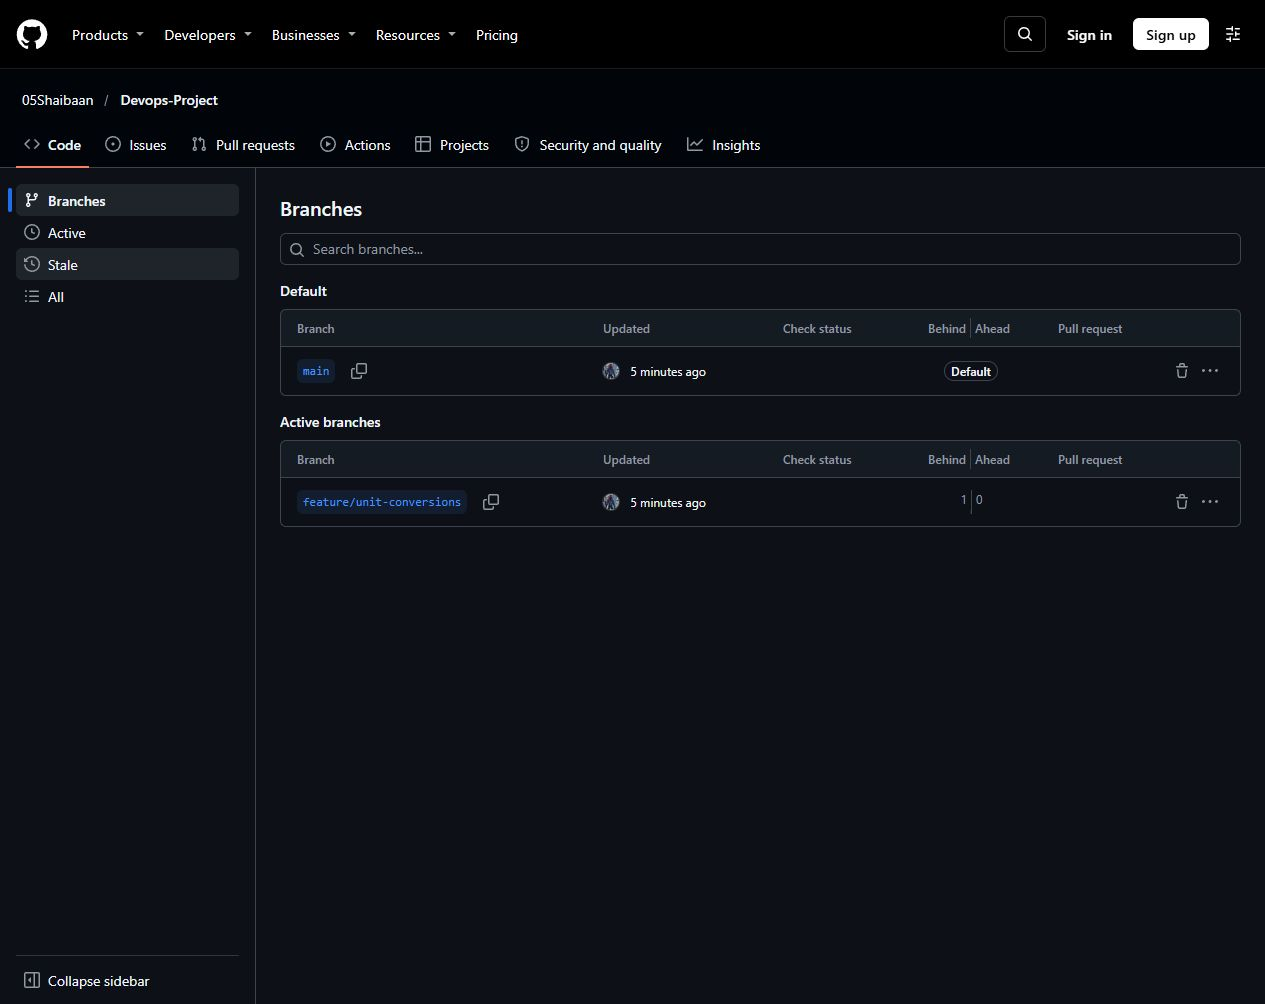
\includegraphics[width=\linewidth,height=0.67\textheight,keepaspectratio]{01-github-branches.jpg}
\par\smallskip The main and feature/unit-conversions branches on GitHub.\end{center}

\begin{center}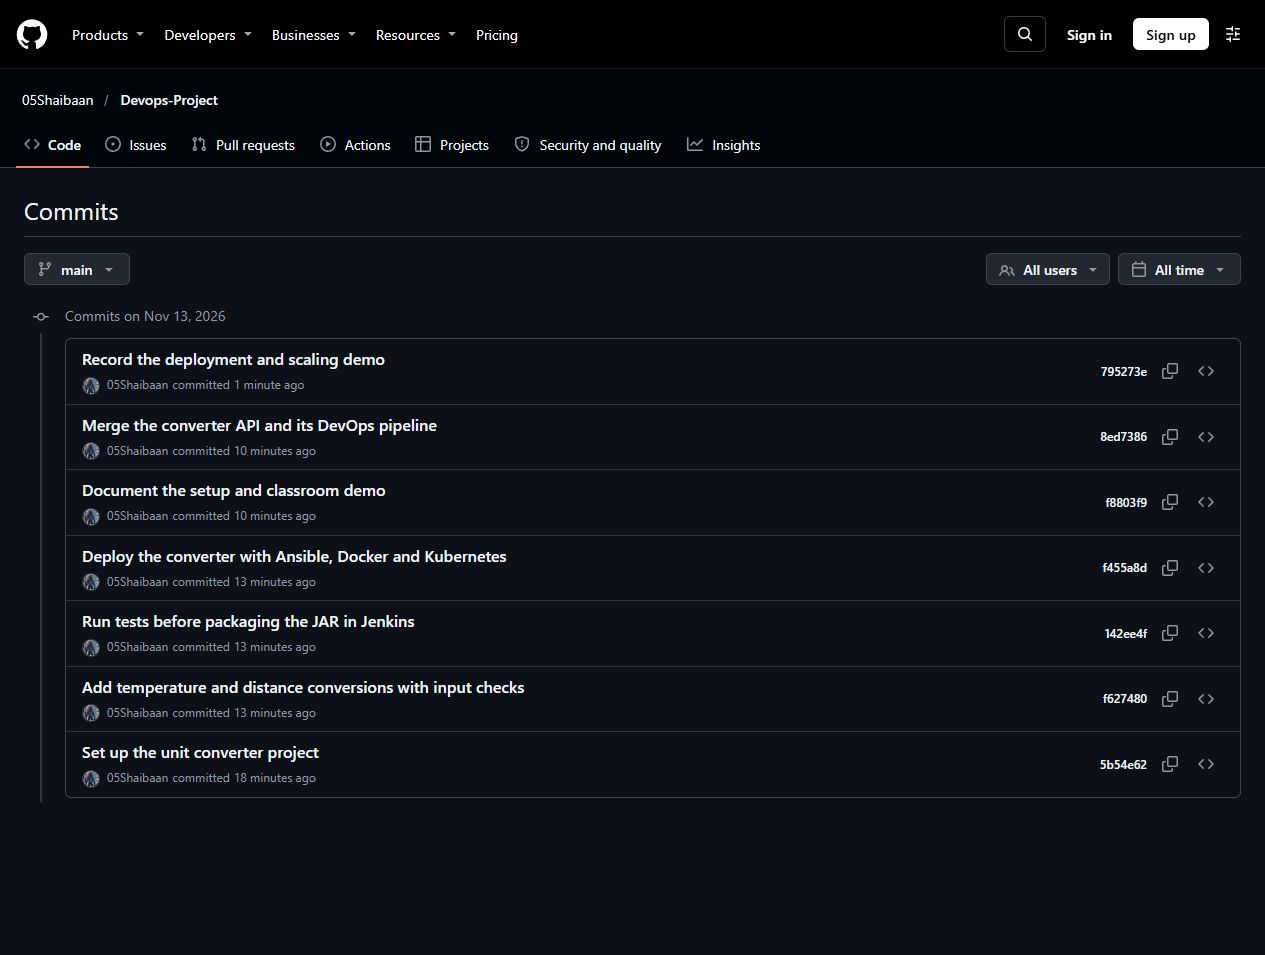
\includegraphics[width=\linewidth,height=0.67\textheight,keepaspectratio]{02-github-merge-history.jpg}
\par\smallskip Commit history includes the feature merge and Shaibaan attribution.\end{center}

\begin{center}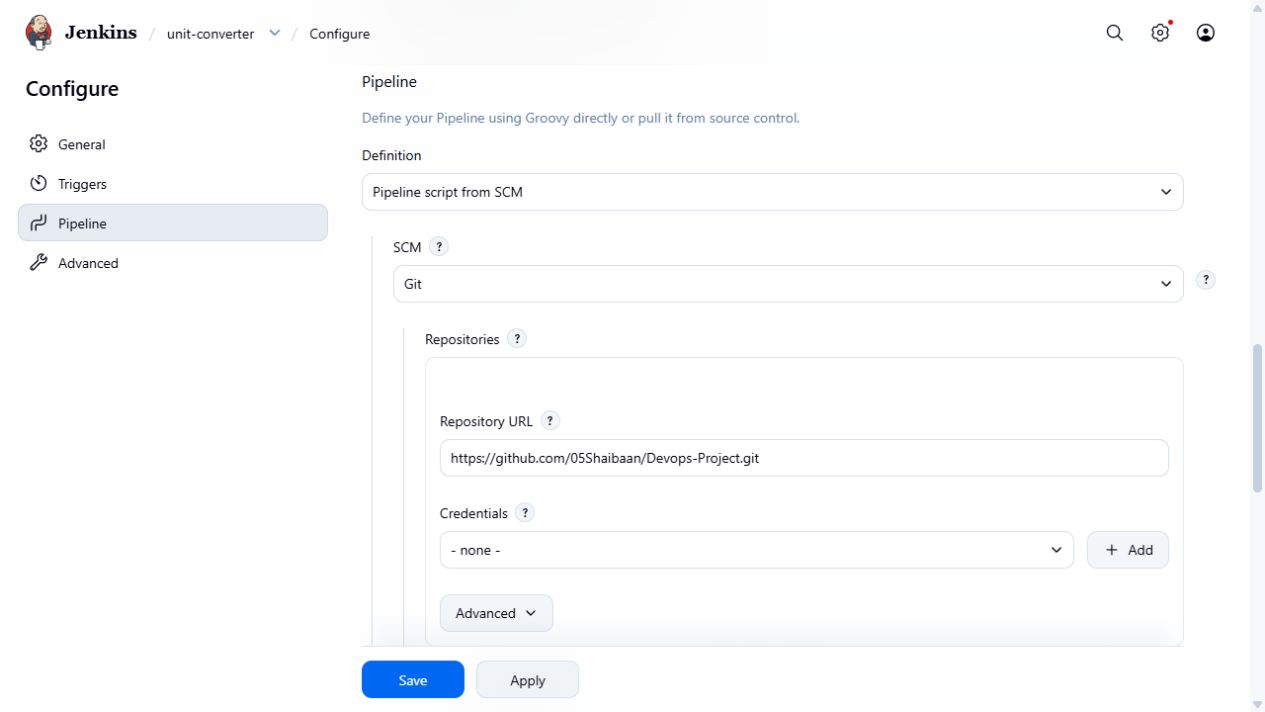
\includegraphics[width=\linewidth,height=0.67\textheight,keepaspectratio]{03-jenkins-repository-configuration.jpg}
\par\smallskip Jenkins reads this repository and the Jenkinsfile from SCM.\end{center}

\begin{center}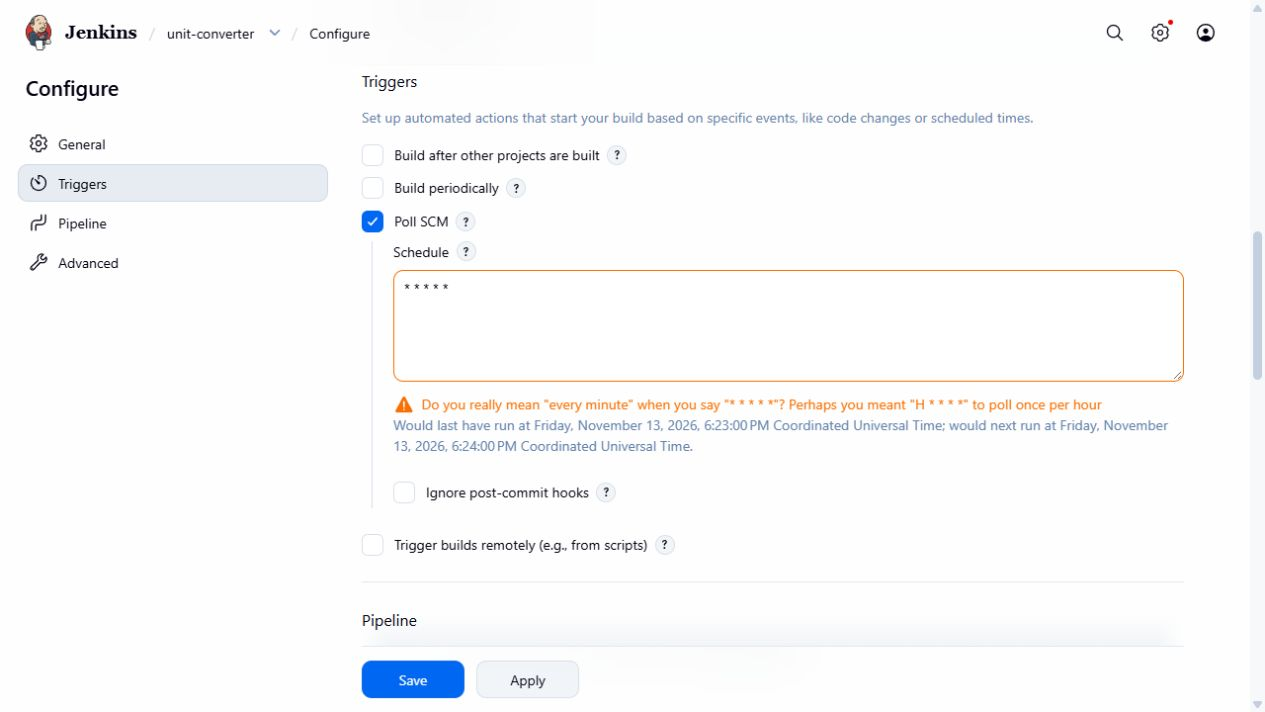
\includegraphics[width=\linewidth,height=0.67\textheight,keepaspectratio]{04-jenkins-scm-trigger.jpg}
\par\smallskip SCM polling checks for new commits every minute.\end{center}

\begin{center}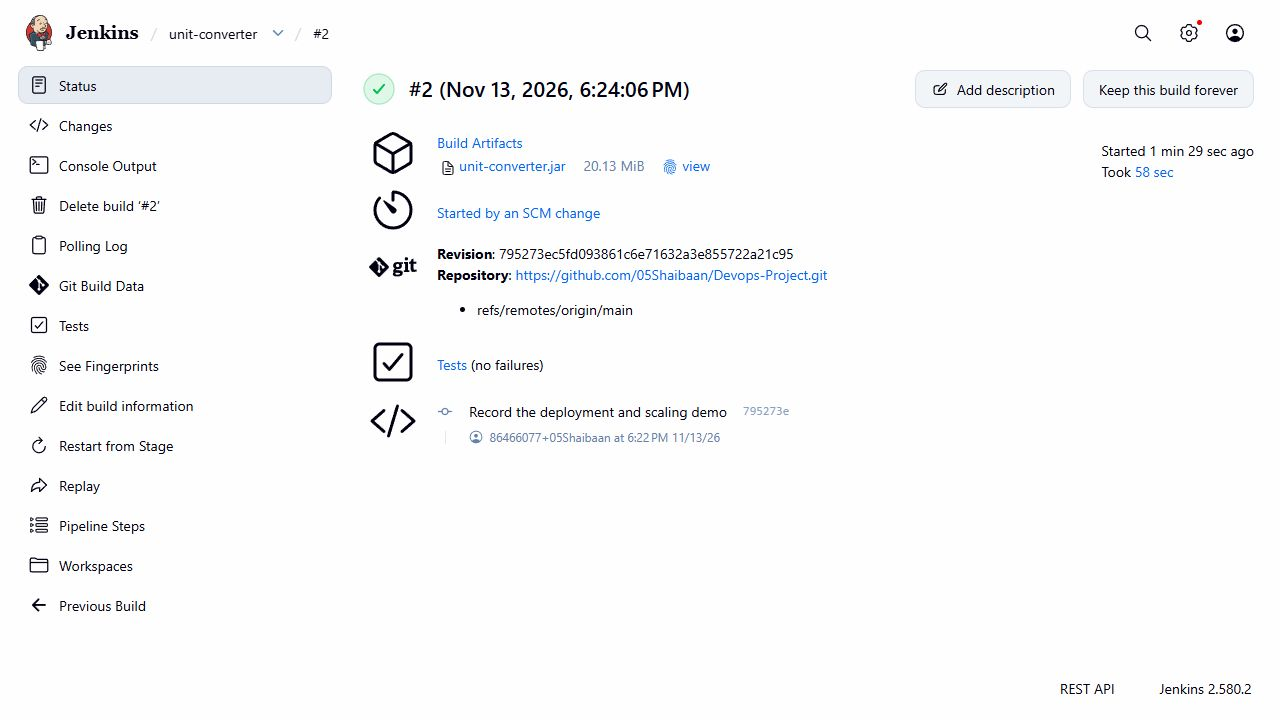
\includegraphics[width=\linewidth,height=0.67\textheight,keepaspectratio]{05-jenkins-successful-pipeline.jpg}
\par\smallskip Successful pipeline triggered automatically by an SCM change.\end{center}

\begin{center}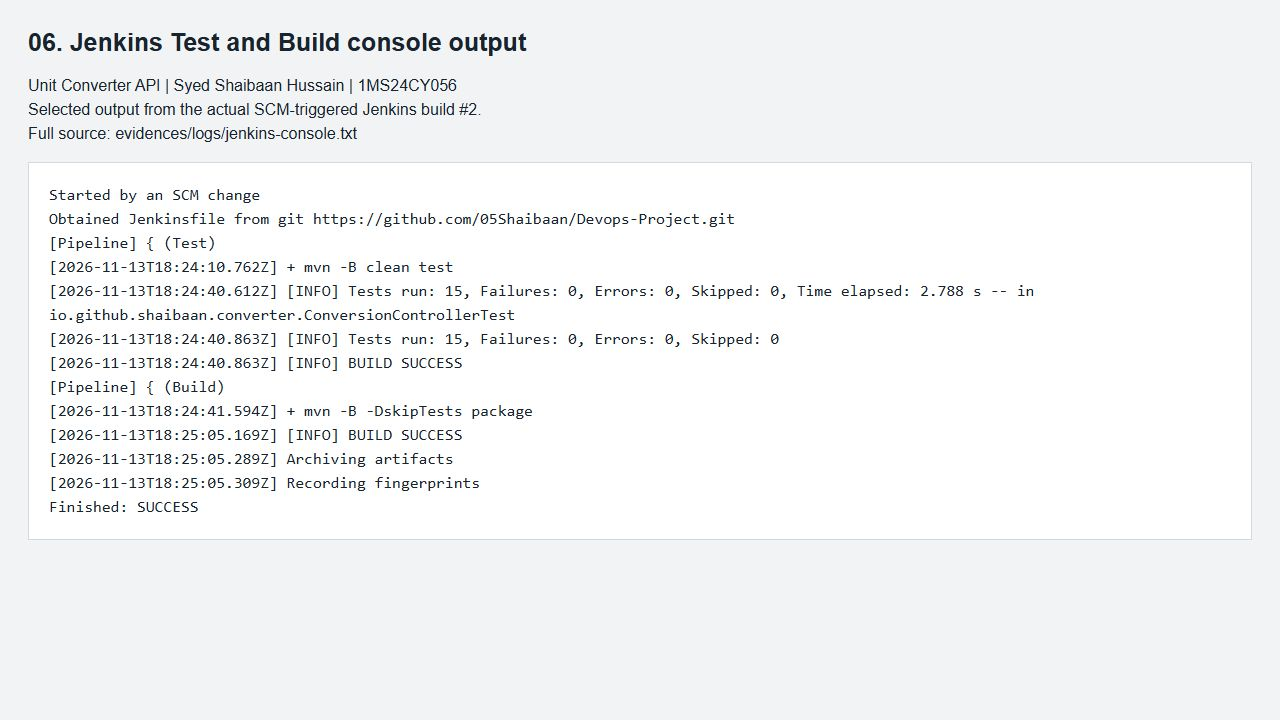
\includegraphics[width=\linewidth,height=0.67\textheight,keepaspectratio]{06-jenkins-test-and-build-console.jpg}
\par\smallskip Console output confirms the tests and packaging completed.\end{center}

\begin{center}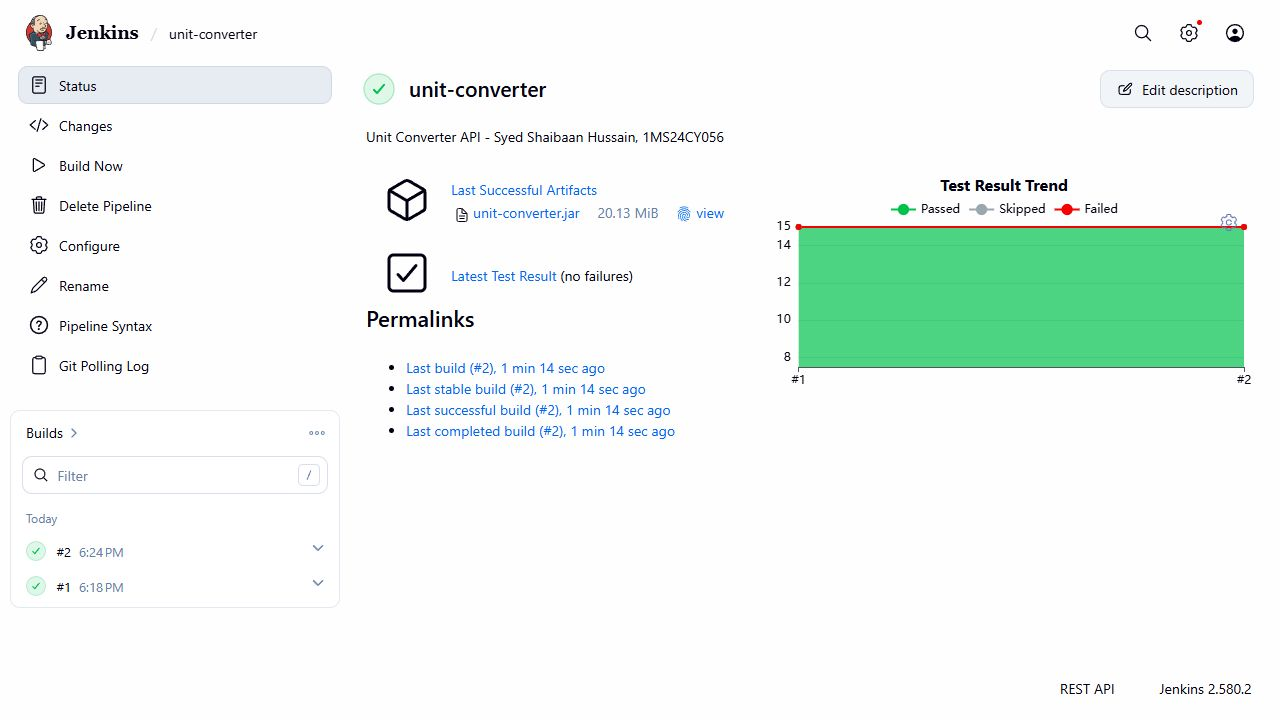
\includegraphics[width=\linewidth,height=0.67\textheight,keepaspectratio]{07-jenkins-archived-jar.jpg}
\par\smallskip Jenkins retains the executable JAR as an archived artifact.\end{center}

\begin{center}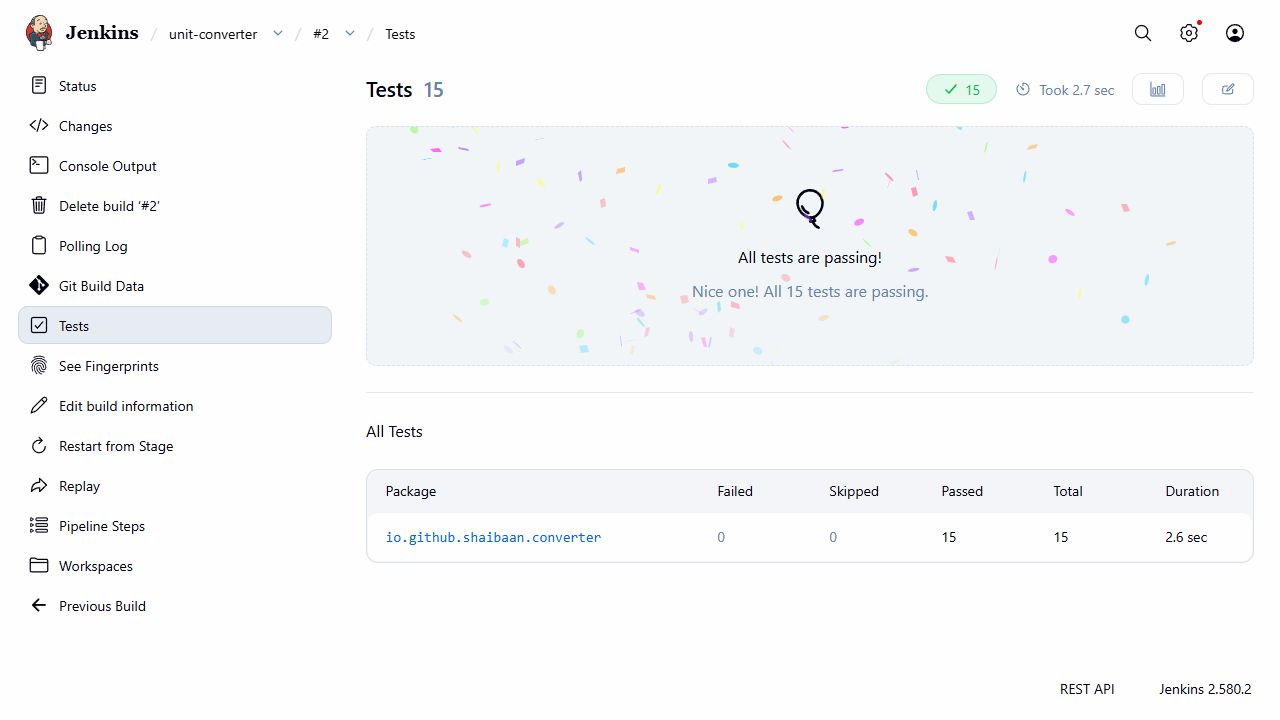
\includegraphics[width=\linewidth,height=0.67\textheight,keepaspectratio]{08-jenkins-passing-tests.jpg}
\par\smallskip All fifteen automated tests passed.\end{center}

\subsection*{Conclusion}

This component produced a working converter and a repeatable build-and-test pipeline. The branch history records the implementation, the automatic SCM build demonstrates CI, and the archived JAR supplies the exact application needed by the next component. Test failures stop packaging and make calculation or validation regressions visible early.

\paragraph{Resume line.} Built a Java Unit Converter API and automated its Maven build in Jenkins with SCM polling, fifteen tests and an archived executable JAR.

\subsection*{References}
\begin{enumerate}
\item Spring Boot servlet web applications: \url{https://docs.spring.io/spring-boot/3.5/reference/web/servlet.html}
\item Maven build lifecycle: \url{https://maven.apache.org/guides/introduction/introduction-to-the-lifecycle.html}
\item Jenkins Pipeline syntax: \url{https://www.jenkins.io/doc/book/pipeline/syntax/}
\item Git branching and merging: \url{https://git-scm.com/book/en/v2/Git-Branching-Basic-Branching-and-Merging}
\end{enumerate}
\newpage
\section*{Component 2: Configuration Management and Kubernetes Deployment}
\subsection*{Abstract}
This component deploys the same Unit Converter API through Ansible, Docker and Kubernetes. Ansible configures an Ubuntu service; Docker packages the built JAR; Kubernetes exposes it through a Service and demonstrates three, five and three replicas. A ConfigMap supplies the application port, while health probes control readiness and detect an unhealthy container.

\subsection*{Introduction}
Configuration management records server setup in a playbook so it can be repeated. A Docker image then packages the runtime and application together. Kubernetes manages copies of that image, replaces failed containers and gives clients a stable Service address. Keeping the API stateless means every replica performs the same calculation without shared storage.

\subsection*{Implementation}
\subsubsection*{Development Environment}
The deployment uses Ubuntu under WSL2, Ansible Core 2.20.1, Docker Engine 29.1.3, Kind 0.31.0 and kubectl 1.35.0. The dedicated cluster is \texttt{converter-demo}; its namespace is also \texttt{converter-demo}. The Ansible service uses port 8093, the container test uses 8095, and the Kubernetes Service is forwarded to 8096, keeping the three demonstrations independent.

\subsubsection*{Ansible Inventory, Playbook and Role}
The inventory targets the local Ubuntu host. The \texttt{converter} role was initialized using \texttt{ansible-galaxy role init converter}. It installs Java 17, creates an unprivileged service account, copies the built JAR, renders the systemd unit and checks the health route. Variables define the port, user, directory and artifact path. Changed files notify a restart handler; unchanged files do not restart the application.

\par\medskip\needspace{4\baselineskip}\noindent\textbf{\path{ansible/inventory}}\par\smallskip

\begin{lstlisting}
[app_servers]
localhost ansible_connection=local
\end{lstlisting}

\par\medskip\needspace{4\baselineskip}\noindent\textbf{\path{ansible/playbook.yml}}\par\smallskip

\begin{lstlisting}
---
- name: Configure the Unit Converter API server
  hosts: app_servers
  become: true
  roles:
    - converter
\end{lstlisting}

\par\medskip\needspace{4\baselineskip}\noindent\textbf{\path{ansible/roles/converter/defaults/main.yml}}\par\smallskip

\begin{lstlisting}
---
app_port: 8093
app_directory: /opt/unit-converter
app_user: unit-converter
app_jar: "{{ playbook_dir }}/../target/unit-converter.jar"
\end{lstlisting}

\par\medskip\needspace{4\baselineskip}\noindent\textbf{\path{ansible/roles/converter/tasks/main.yml}}\par\smallskip

\begin{lstlisting}
---
- name: Install the Java runtime
  ansible.builtin.apt:
    name: openjdk-17-jre-headless
    state: present
    update_cache: true
    cache_valid_time: 3600

- name: Create a service account
  ansible.builtin.user:
    name: "{{ app_user }}"
    system: true
    shell: /usr/sbin/nologin
    create_home: false

- name: Create the application directory
  ansible.builtin.file:
    path: "{{ app_directory }}"
    state: directory
    owner: "{{ app_user }}"
    group: "{{ app_user }}"
    mode: '0755'

- name: Copy the built application
  ansible.builtin.copy:
    src: "{{ app_jar }}"
    dest: "{{ app_directory }}/unit-converter.jar"
    owner: "{{ app_user }}"
    group: "{{ app_user }}"
    mode: '0644'
  notify: Restart unit converter

- name: Install the service definition
  ansible.builtin.template:
    src: unit-converter.service.j2
    dest: /etc/systemd/system/unit-converter.service
    mode: '0644'
  notify: Restart unit converter

- name: Apply pending service changes
  ansible.builtin.meta: flush_handlers

- name: Enable and start the service
  ansible.builtin.systemd_service:
    name: unit-converter
    enabled: true
    state: started
    daemon_reload: true

- name: Wait for the API to become healthy
  ansible.builtin.uri:
    url: "http://127.0.0.1:{{ app_port }}/health"
    return_content: true
  register: health
  until: health.status == 200 and health.json.status == 'UP'
  retries: 20
  delay: 3
\end{lstlisting}

\par\medskip\needspace{4\baselineskip}\noindent\textbf{\path{ansible/roles/converter/handlers/main.yml}}\par\smallskip

\begin{lstlisting}
---
- name: Restart unit converter
  ansible.builtin.systemd_service:
    name: unit-converter
    state: restarted
    daemon_reload: true
\end{lstlisting}

\par\medskip\needspace{4\baselineskip}\noindent\textbf{\path{ansible/roles/converter/templates/unit-converter.service.j2}}\par\smallskip

\begin{lstlisting}
[Unit]
Description=Unit Converter API
After=network.target

[Service]
User={{ app_user }}
Group={{ app_user }}
WorkingDirectory={{ app_directory }}
Environment=APP_PORT={{ app_port }}
ExecStart=/usr/bin/java -jar {{ app_directory }}/unit-converter.jar
Restart=on-failure
RestartSec=5
NoNewPrivileges=true
PrivateTmp=true
ProtectSystem=strict
ProtectHome=true
TimeoutStopSec=20

[Install]
WantedBy=multi-user.target
\end{lstlisting}

\subsubsection*{Docker Image and Local Container}

The image uses the Java 17 runtime, copies the executable JAR and starts it as user 10001. The build context contains only the packaged artifact. A local container was started with a loopback port mapping and checked with the distance route before the image was loaded into Kind.

\par\medskip\needspace{4\baselineskip}\noindent\textbf{\path{Dockerfile}}\par\smallskip

\begin{lstlisting}
FROM eclipse-temurin:17-jre-jammy
WORKDIR /app
COPY --chown=10001:10001 target/unit-converter.jar app.jar
USER 10001:10001
EXPOSE 8080
ENTRYPOINT ["java", "-XX:MaxRAMPercentage=75.0", "-jar", "app.jar"]
\end{lstlisting}

\par\medskip\needspace{4\baselineskip}\noindent\textbf{\path{.dockerignore}}\par\smallskip

\begin{lstlisting}
**
!target/
!target/unit-converter.jar
\end{lstlisting}

\subsubsection*{Kubernetes Deployment and Service}

The Deployment requests three replicas of \texttt{unit-converter:1.0}. Its pod label and Service selector both use \texttt{app: unit-converter}. The ClusterIP Service maps port 8080 to the named HTTP container port. Resource requests and limits keep the local demonstration bounded. The namespace and ConfigMap are created before the application is started.

\par\medskip\needspace{4\baselineskip}\noindent\textbf{\path{k8s/namespace.yaml}}\par\smallskip

\begin{lstlisting}
apiVersion: v1
kind: Namespace
metadata:
  name: converter-demo
\end{lstlisting}

\par\medskip\needspace{4\baselineskip}\noindent\textbf{\path{k8s/deployment.yaml}}\par\smallskip

\begin{lstlisting}
apiVersion: apps/v1
kind: Deployment
metadata:
  namespace: converter-demo
  name: unit-converter
spec:
  replicas: 3
  selector:
    matchLabels:
      app: unit-converter
  template:
    metadata:
      labels:
        app: unit-converter
    spec:
      securityContext:
        runAsNonRoot: true
        runAsUser: 10001
        runAsGroup: 10001
      containers:
        - name: unit-converter
          image: unit-converter:1.0
          imagePullPolicy: IfNotPresent
          envFrom:
            - configMapRef:
                name: unit-converter-config
          ports:
            - name: http
              containerPort: 8080
          resources:
            requests:
              cpu: 100m
              memory: 192Mi
            limits:
              cpu: 500m
              memory: 384Mi
          securityContext:
            allowPrivilegeEscalation: false
            capabilities:
              drop: [ALL]
          startupProbe:
            httpGet:
              path: /health
              port: http
            periodSeconds: 5
            failureThreshold: 30
          readinessProbe:
            httpGet:
              path: /health
              port: http
            periodSeconds: 5
          livenessProbe:
            httpGet:
              path: /health
              port: http
            periodSeconds: 10
\end{lstlisting}

\par\medskip\needspace{4\baselineskip}\noindent\textbf{\path{k8s/service.yaml}}\par\smallskip

\begin{lstlisting}
apiVersion: v1
kind: Service
metadata:
  namespace: converter-demo
  name: unit-converter
spec:
  selector:
    app: unit-converter
  ports:
    - name: http
      port: 8080
      targetPort: http
  type: ClusterIP
\end{lstlisting}

\par\medskip\needspace{4\baselineskip}\noindent\textbf{\path{scripts/deploy.sh}}\par\smallskip

\begin{lstlisting}[language=bash]
#!/usr/bin/env bash
set -euo pipefail
cd "$(dirname "$0")/.."

# Use the dedicated demo cluster so another Kubernetes context is never changed.
kind load docker-image unit-converter:1.0 --name converter-demo
kubectl --context kind-converter-demo apply -f k8s/namespace.yaml
kubectl --context kind-converter-demo -n converter-demo apply -f k8s/
kubectl --context kind-converter-demo -n converter-demo rollout status deployment/unit-converter --timeout=180s
kubectl --context kind-converter-demo -n converter-demo get pods -l app=unit-converter
kubectl --context kind-converter-demo -n converter-demo get service unit-converter
\end{lstlisting}

\subsubsection*{Scaling}

The application starts with three ready replicas. Scaling to five adds two pods; scaling back to three removes them. The script waits for rollout completion and the reported replica count at each step. This demonstrates manual horizontal scaling; it does not claim an autoscaler was installed.

\par\medskip\needspace{4\baselineskip}\noindent\textbf{\path{scripts/scale-demo.sh}}\par\smallskip

\begin{lstlisting}[language=bash]
#!/usr/bin/env bash
set -euo pipefail

for replicas in 3 5 3; do
    echo "Scaling unit-converter to $replicas replicas"
    kubectl --context kind-converter-demo -n converter-demo scale deployment/unit-converter --replicas="$replicas"
    kubectl --context kind-converter-demo -n converter-demo rollout status deployment/unit-converter --timeout=180s
    kubectl --context kind-converter-demo -n converter-demo wait deployment/unit-converter \
        --for="jsonpath={.status.replicas}=$replicas" --timeout=180s
    kubectl --context kind-converter-demo -n converter-demo get pods -l app=unit-converter
done
\end{lstlisting}

\subsection*{Enhancement: ConfigMap and Health Probes}

The ConfigMap supplies \texttt{APP\_PORT=8080} through the Deployment\textquotesingle s \texttt{envFrom}. This separates an application setting from the image. The startup probe allows time for Java to start, readiness keeps traffic away until the API responds, and liveness allows Kubernetes to restart an unhealthy container. All three use \texttt{/health}. Changing environment settings requires restarting the pods; changing the listening port also requires matching the container port and probes.

\par\medskip\needspace{4\baselineskip}\noindent\textbf{\path{k8s/configmap.yaml}}\par\smallskip

\begin{lstlisting}
apiVersion: v1
kind: ConfigMap
metadata:
  namespace: converter-demo
  name: unit-converter-config
data:
  APP_PORT: "8080"
\end{lstlisting}

\subsection*{Description of the Activity}

The Ansible playbook first installed the service and successfully checked its response. A second unchanged run confirmed idempotence. The same JAR was built into a Docker image and tested locally. That image was loaded into a separate Kind cluster, the manifests were applied, and the Service was checked with both conversion routes. Replicas were increased to five and returned to three. Finally, the container environment was inspected to confirm that the ConfigMap value reached the running application.

\subsection*{Results}

Ansible completed with zero unreachable or failed hosts; the repeated run reported zero changes. Docker built the image and returned 3.1069 miles for 5 kilometres. The Kind node became Ready, and Kubernetes showed three, five and three ready pods. Service requests returned 77 Fahrenheit and 3.1069 miles. The running container reported \texttt{APP\_PORT=8080}. Screenshots 09--21 display actual recorded command output; the complete logs are included in the repository.

\begin{center}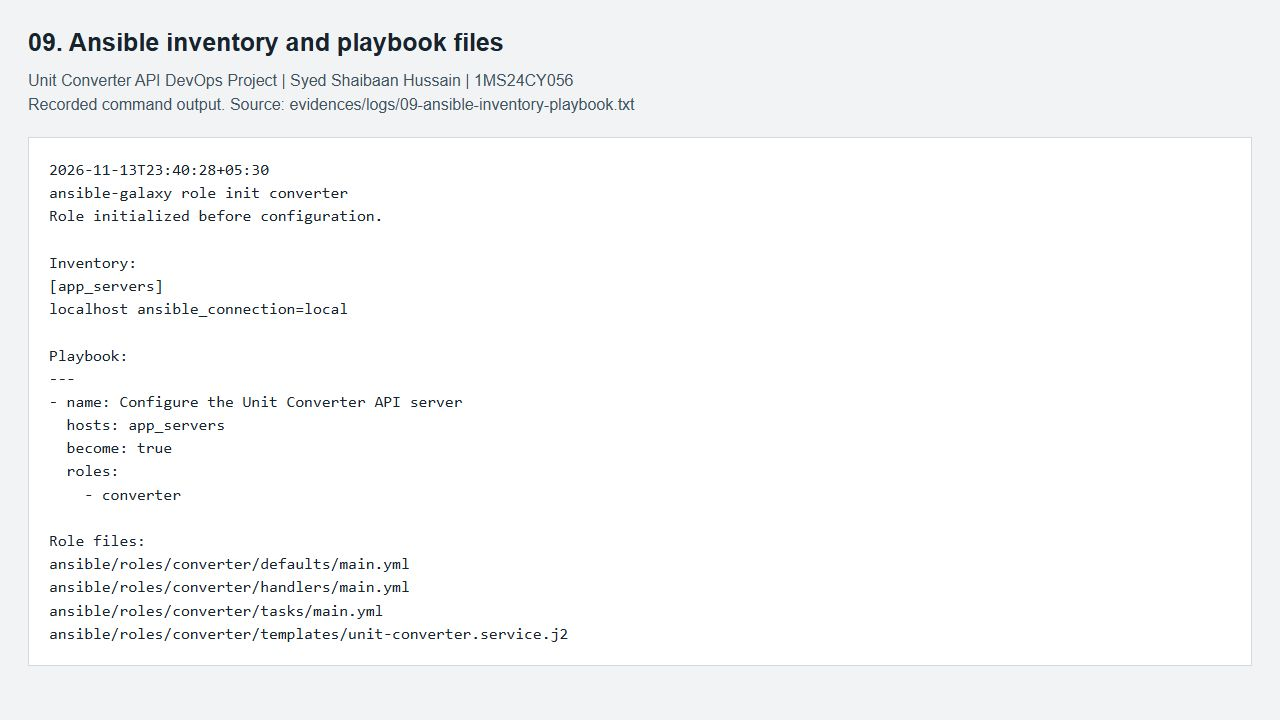
\includegraphics[width=\linewidth,height=0.67\textheight,keepaspectratio]{09-ansible-inventory-playbook.jpg}
\par\smallskip Inventory, playbook and initialized role files.\end{center}

\begin{center}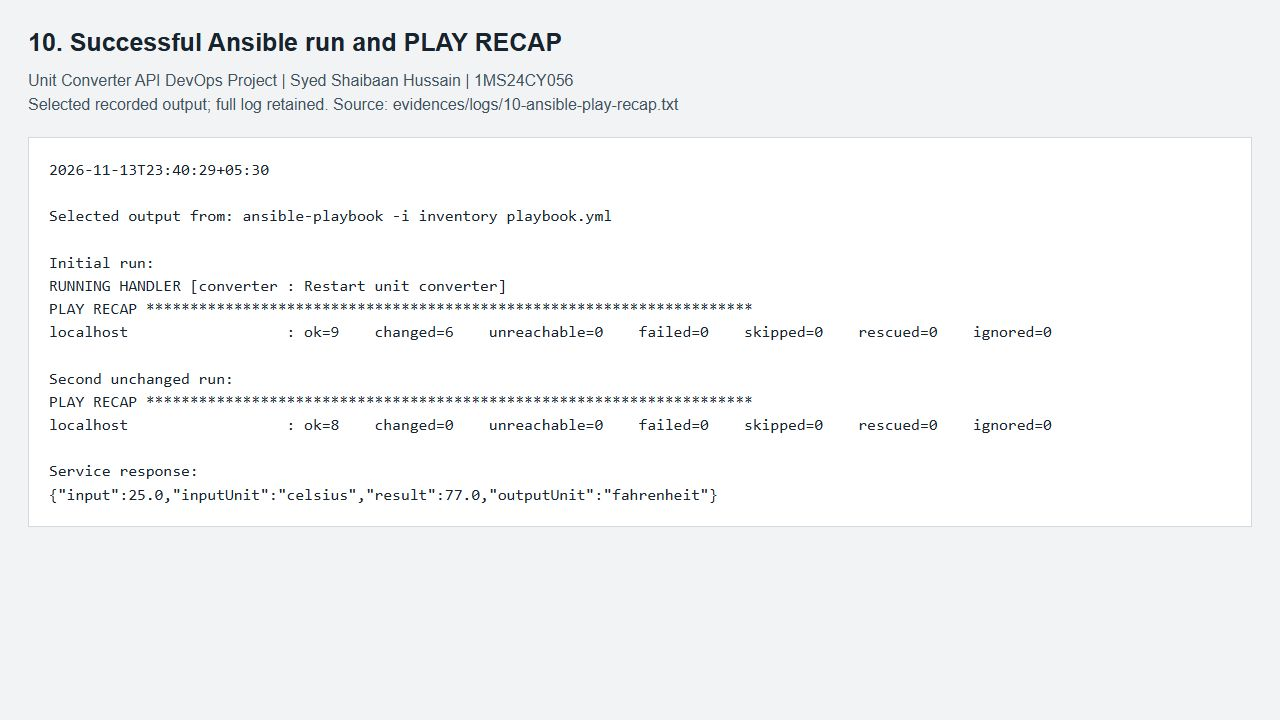
\includegraphics[width=\linewidth,height=0.67\textheight,keepaspectratio]{10-ansible-play-recap.jpg}
\par\smallskip Successful Ansible execution and unchanged second run.\end{center}

\begin{center}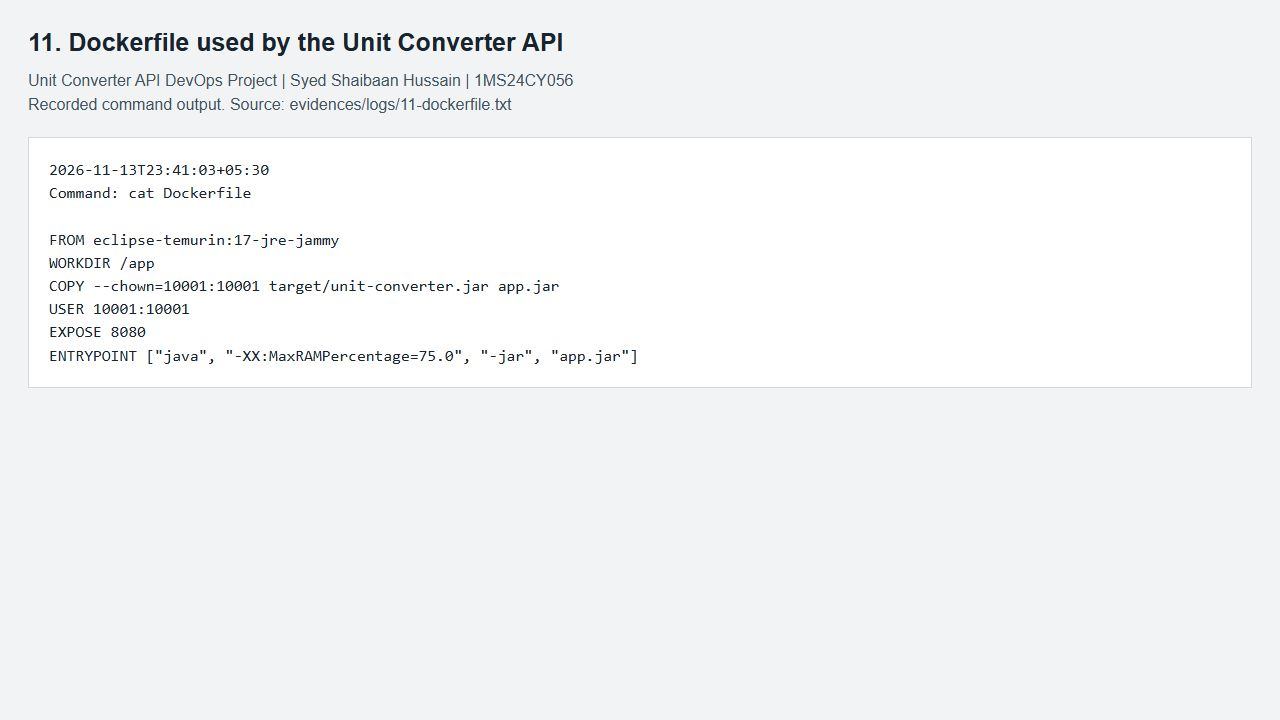
\includegraphics[width=\linewidth,height=0.67\textheight,keepaspectratio]{11-dockerfile.jpg}
\par\smallskip Dockerfile used to package the JAR.\end{center}

\begin{center}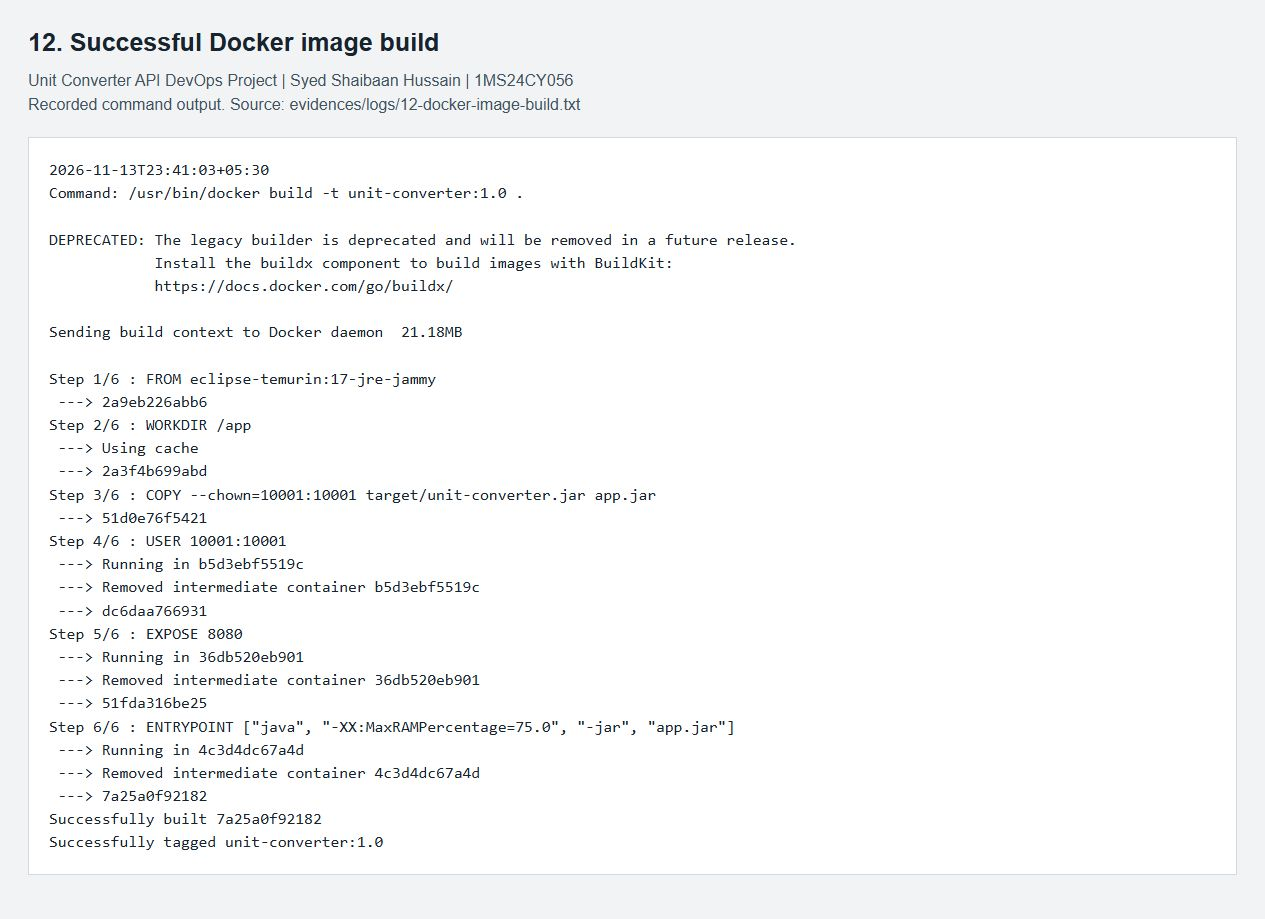
\includegraphics[width=\linewidth,height=0.67\textheight,keepaspectratio]{12-docker-image-build.jpg}
\par\smallskip Docker image build completed successfully.\end{center}

\begin{center}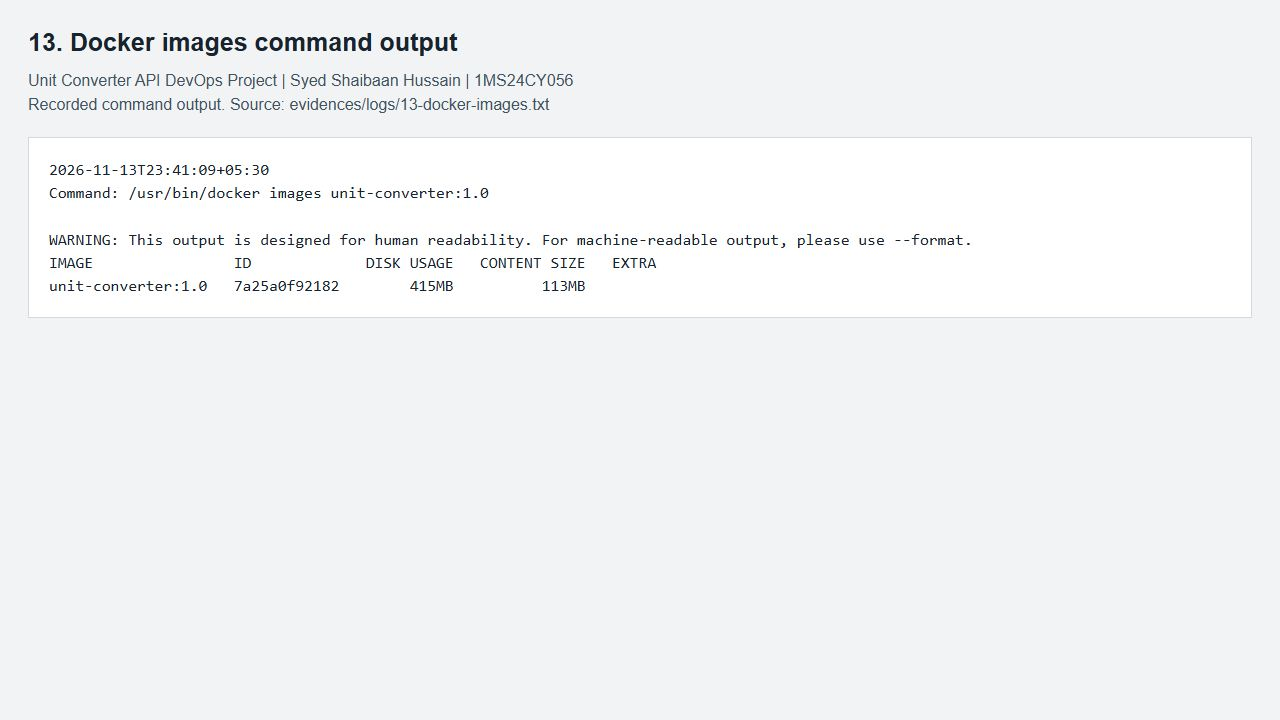
\includegraphics[width=\linewidth,height=0.67\textheight,keepaspectratio]{13-docker-images.jpg}
\par\smallskip Built unit-converter image in the local image list.\end{center}

\begin{center}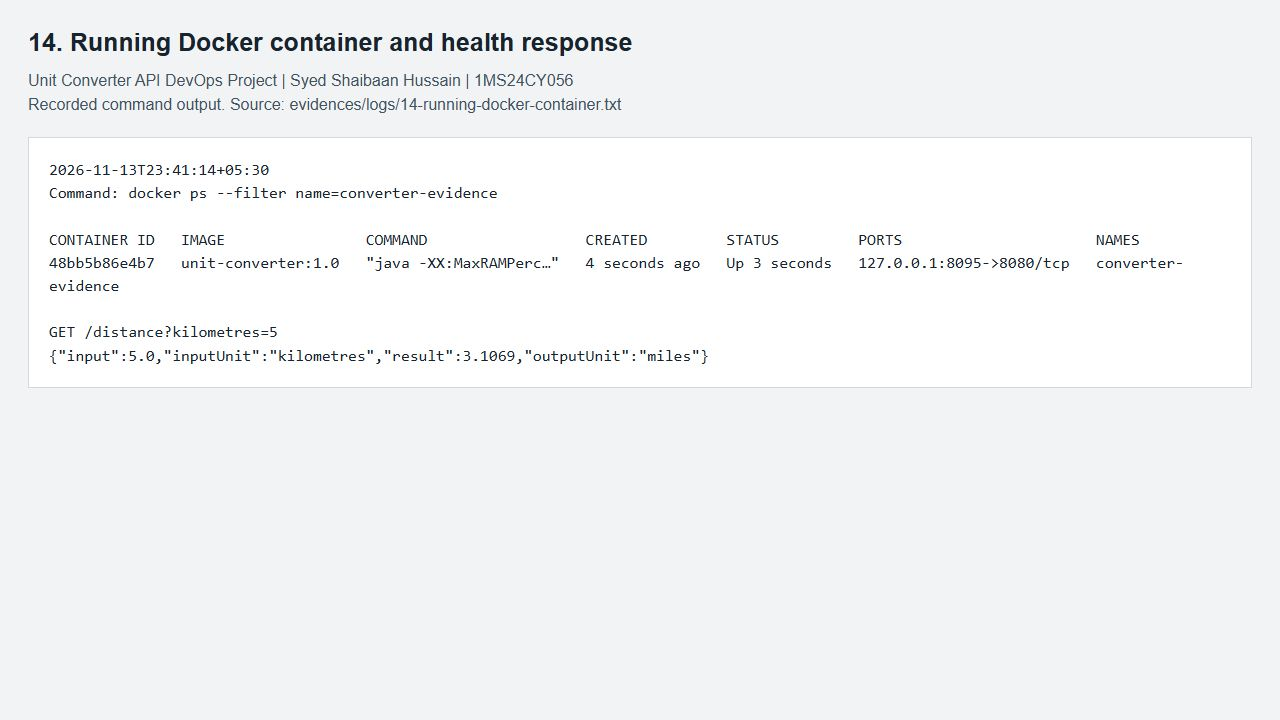
\includegraphics[width=\linewidth,height=0.67\textheight,keepaspectratio]{14-running-docker-container.jpg}
\par\smallskip Running container returns the distance conversion.\end{center}

\begin{center}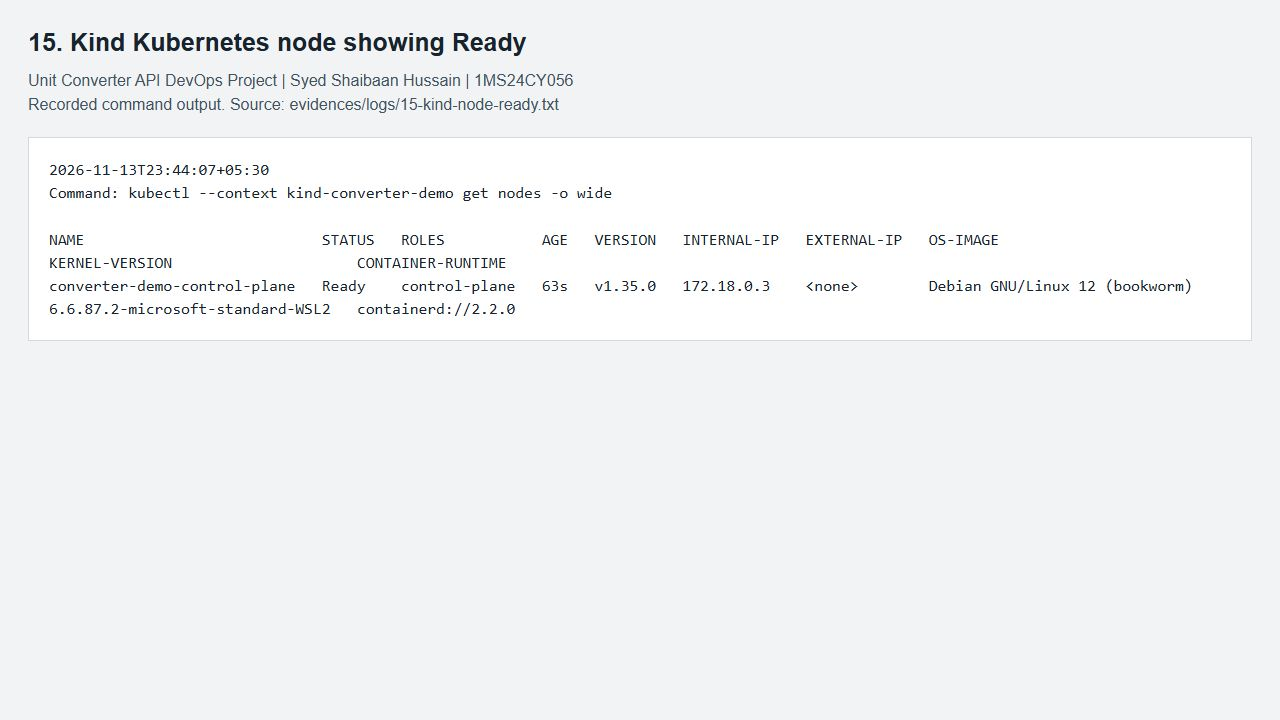
\includegraphics[width=\linewidth,height=0.67\textheight,keepaspectratio]{15-kind-node-ready.jpg}
\par\smallskip The dedicated Kind control-plane node is Ready.\end{center}

\begin{center}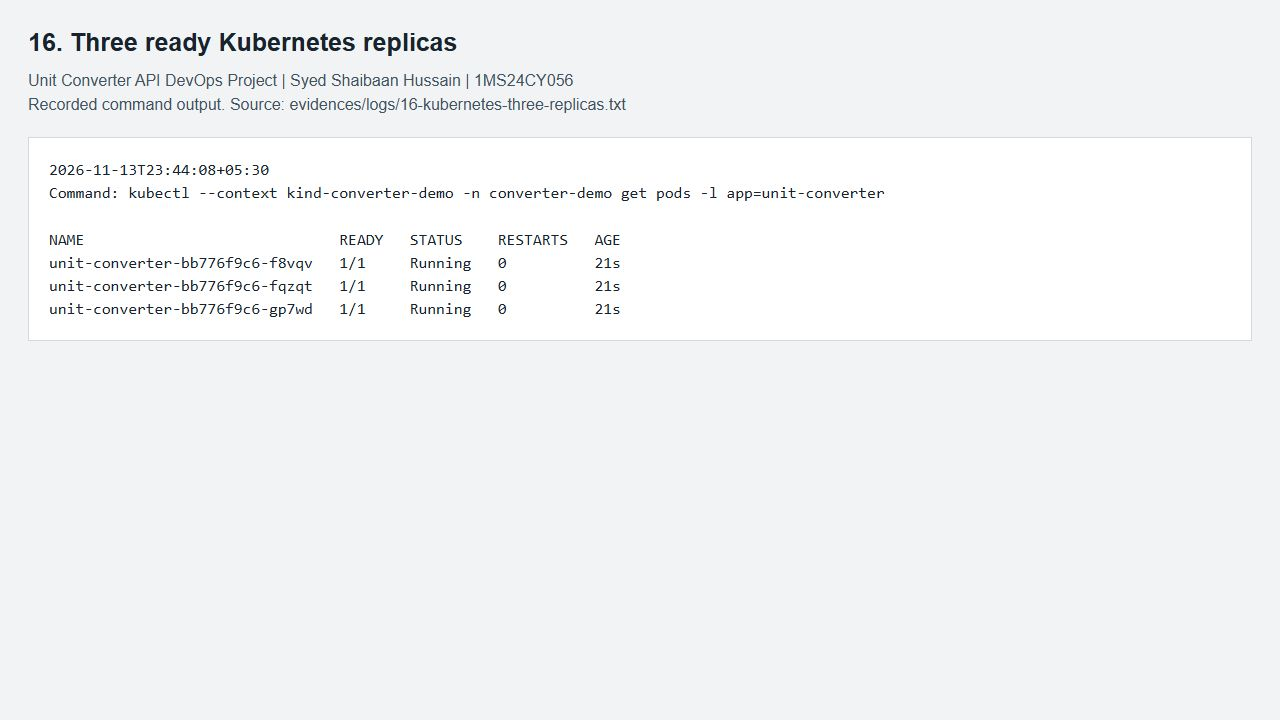
\includegraphics[width=\linewidth,height=0.67\textheight,keepaspectratio]{16-kubernetes-three-replicas.jpg}
\par\smallskip Three initial replicas are ready.\end{center}

\begin{center}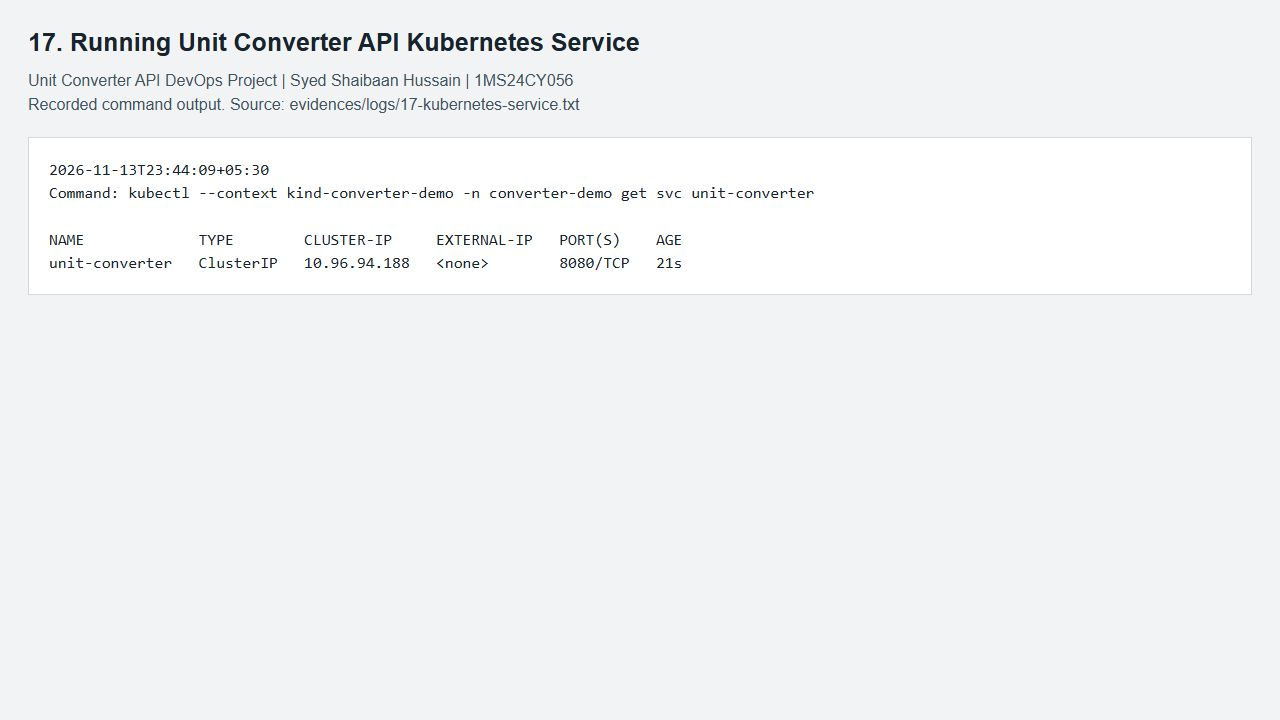
\includegraphics[width=\linewidth,height=0.67\textheight,keepaspectratio]{17-kubernetes-service.jpg}
\par\smallskip The ClusterIP Service exposes the converter.\end{center}

\begin{center}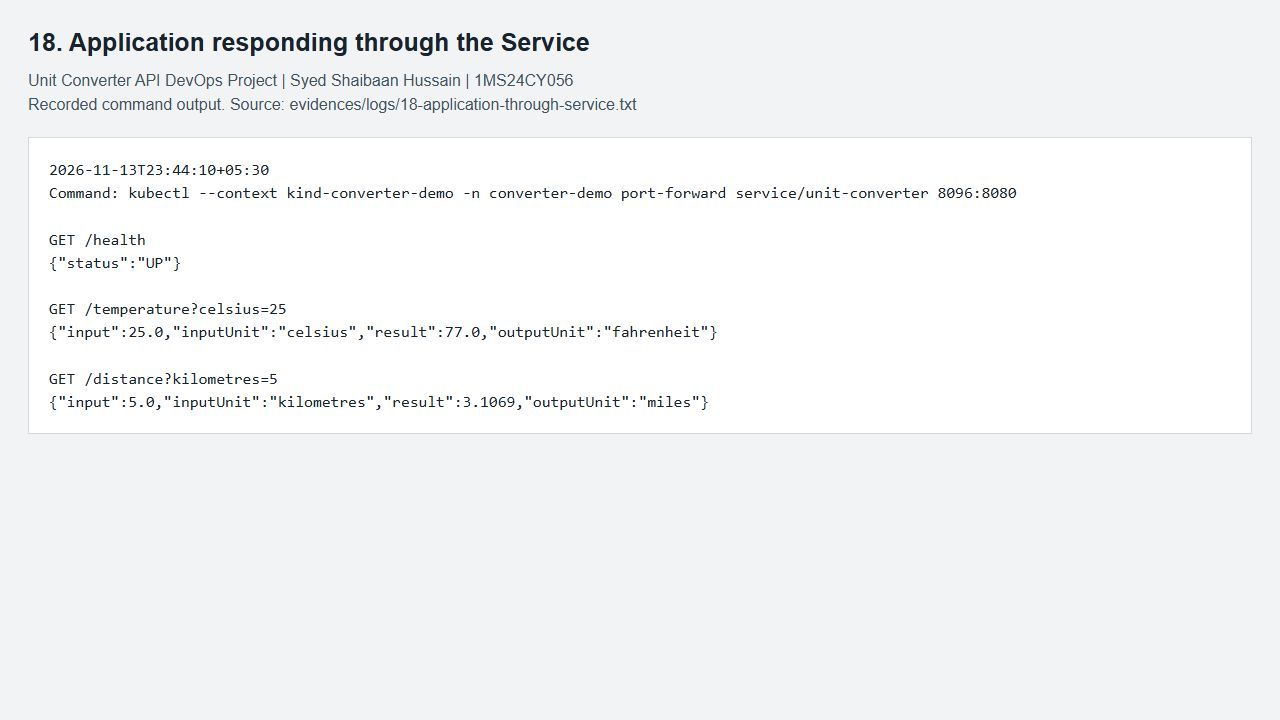
\includegraphics[width=\linewidth,height=0.67\textheight,keepaspectratio]{18-application-through-service.jpg}
\par\smallskip Application responses through the Kubernetes Service.\end{center}

\begin{center}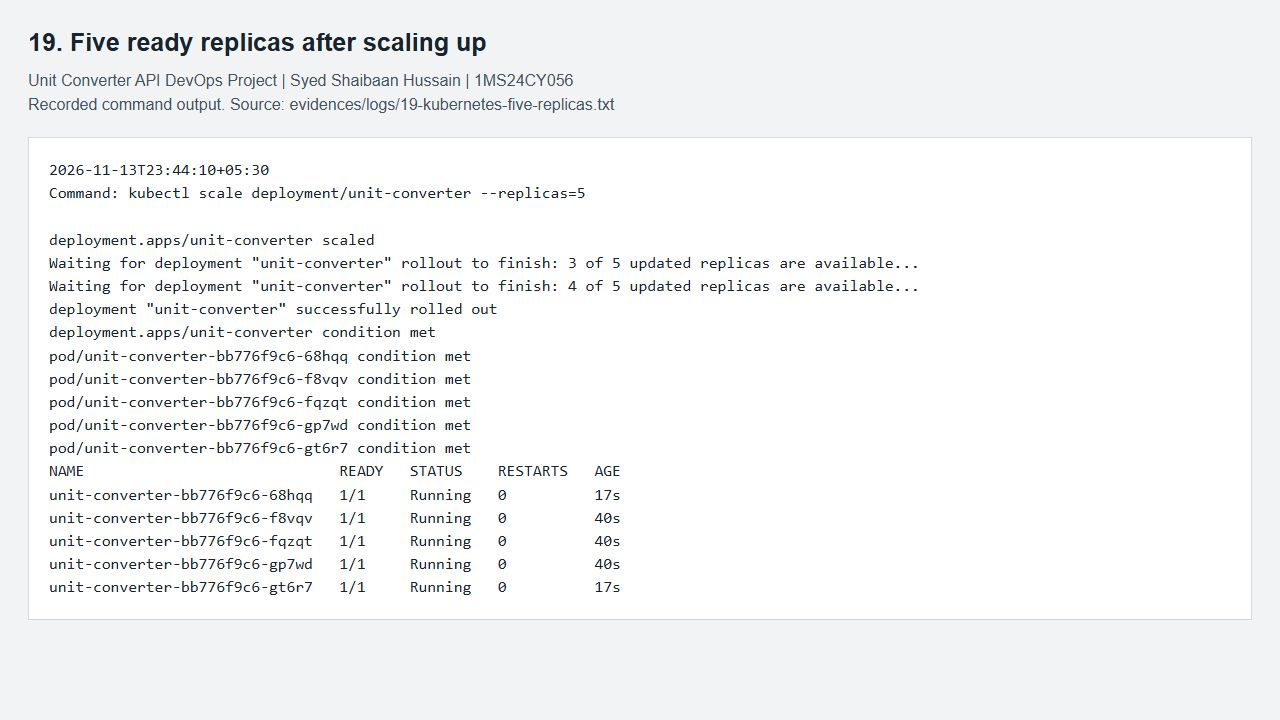
\includegraphics[width=\linewidth,height=0.67\textheight,keepaspectratio]{19-kubernetes-five-replicas.jpg}
\par\smallskip Five ready replicas after scaling up.\end{center}

\begin{center}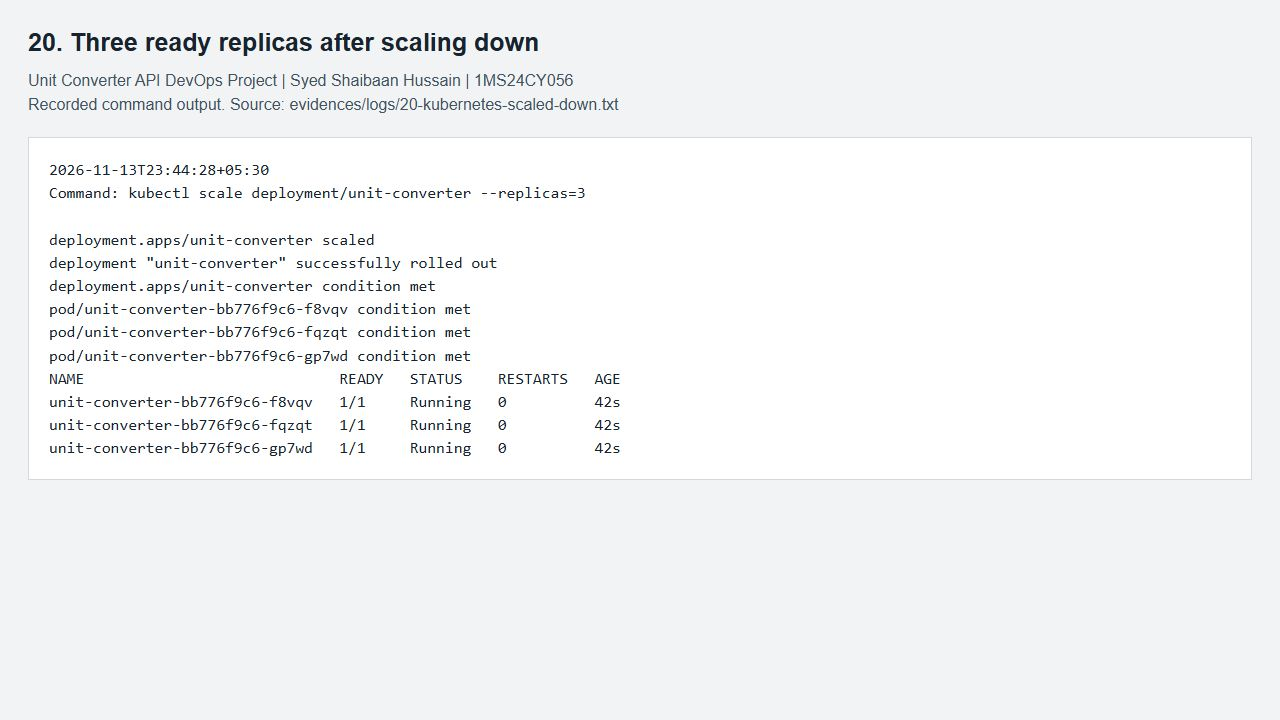
\includegraphics[width=\linewidth,height=0.67\textheight,keepaspectratio]{20-kubernetes-scaled-down.jpg}
\par\smallskip Three ready replicas after scaling down.\end{center}

\begin{center}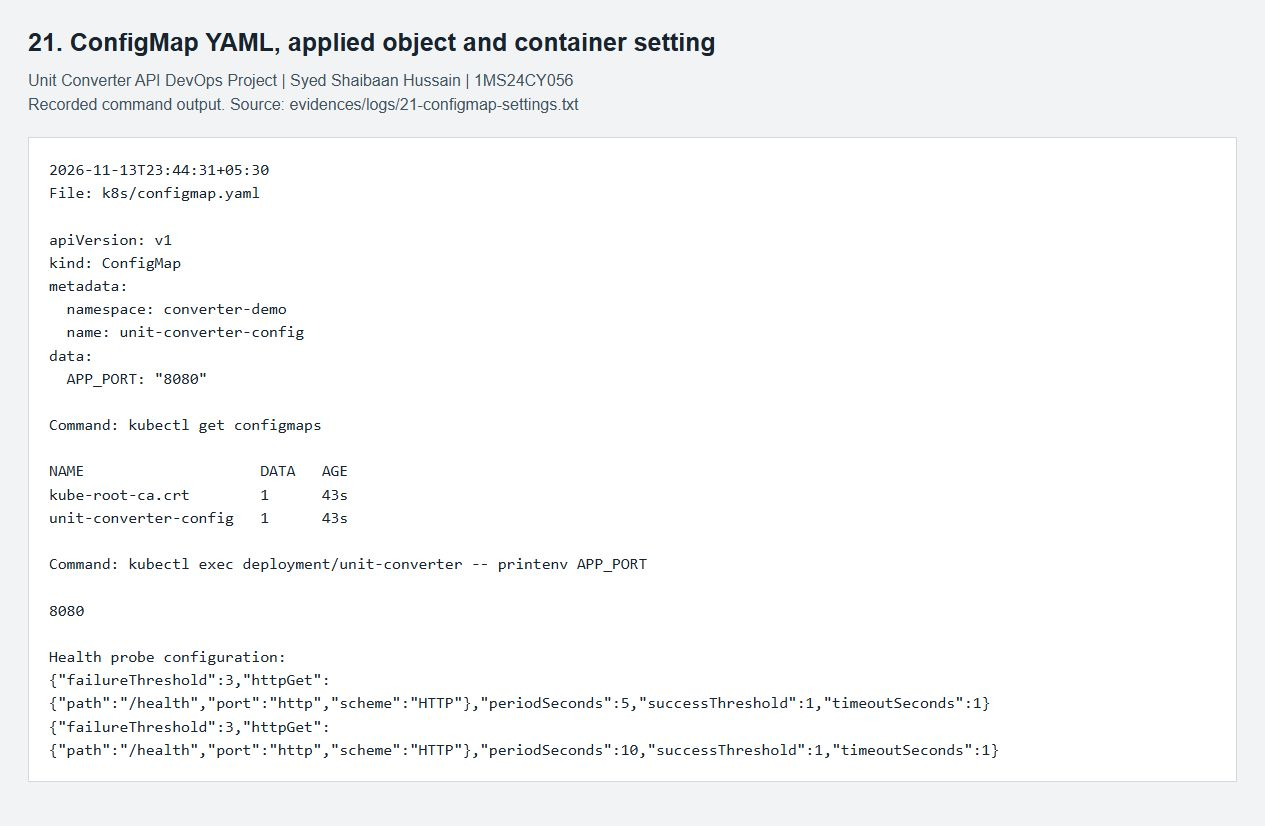
\includegraphics[width=\linewidth,height=0.67\textheight,keepaspectratio]{21-configmap-settings.jpg}
\par\smallskip ConfigMap value in the container and health probe configuration.\end{center}

\subsection*{Conclusion}

The deployment component demonstrated repeatable server setup, a working container image and a Kubernetes Service with controlled scaling. The ConfigMap and probes make configuration and application health visible. The result remains a small local demonstration with no database, paid cloud service or additional microservice.

\paragraph{Resume line.} Configured an Ubuntu service with an Ansible role and restart handler, then deployed its Docker image on Kubernetes with 3--5--3 scaling, a ConfigMap and health probes.

\subsection*{References}
\begin{enumerate}
\item Ansible roles: \url{https://docs.ansible.com/ansible/latest/playbook_guide/playbooks_reuse_roles.html}
\item Docker build concepts: \url{https://docs.docker.com/build/concepts/dockerfile/}
\item Kind quick start: \url{https://kind.sigs.k8s.io/docs/user/quick-start/}
\item Kubernetes Deployments: \url{https://kubernetes.io/docs/concepts/workloads/controllers/deployment/}
\item ConfigMaps: \url{https://kubernetes.io/docs/concepts/configuration/configmap/}
\item Health probes: \url{https://kubernetes.io/docs/tasks/configure-pod-container/configure-liveness-readiness-startup-probes/}
\end{enumerate}
\paragraph{Submission details.} Repository: \url{https://github.com/05Shaibaan/Devops-Project}. Student: Syed Shaibaan Hussain, USN 1MS24CY056. Candidate and faculty signatures are left for the appropriate signatories, and assessment marks are left for evaluation. The coordinator must be added as a collaborator once their GitHub username is available. The course code follows the assignment brief, 25CYAEC59; the supplied template used 24CYAEC59, so the coordinator should confirm the applicable code before submission.
\end{document}
